% !TEX encoding = UTF-8 Unicode
%!TEX root = thesis.tex
% !TEX spellcheck = en-US
%%=========================================
\section{Experiment 1}
In this experiment, the toolkit is used to make white noise sound like a drum loop that consists of bass drum and snare drum hits. The mfcc\_0 feature is used as neural input and similarity measure. mfcc\_0 measures the spectral energy, so it is expected that the amplitude of the output sound will resemble the amplitude of the drum loop sound. Further, three different output activation functions will be compared.

\subsection{Configuration}
\begin{minipage}{\linewidth}
\centering
\captionof{table}{Table Title TODO} \label{tab:title} 
\begin{tabular}{ C{3.5in} C{1.6in} }\toprule[1.5pt]
\bf Parameter & \bf Value \\
\midrule
  Number of generationa & 10 \\
\midrule
  Fitness function & Local similarity \\
\midrule
  Target sound & Drum loop \\
\midrule
  Input sound & White noise \\
\midrule
  Effect & Distortion and resonant low-pass filter \\
\midrule
  Audio features & mfcc\_0 \\
\midrule
  Output activation function & [Sigmoid, Linear, Sine] \\
\bottomrule[1.25pt]
\end {tabular}\par
\bigskip
Should be a caption TODO
\end{minipage}

\subsection{Fitness function}
The local similarity fitness function is based on the average euclidean distance between the feature vector of the target sound and the output sound in the k frames of the two sounds.

\begin{verbatim}
Function LOCAL_SIMILARITY(target, individual):
    total_euclidean_distance = 0
    for each k in range(num_frames):
        A = target.get_feature_vector(k)
        C = individual.get_feature_vector(k)
        total_euclidean_distance += EUCLIDEAN_DISTANCE(A, C)
    avg_euclidean_distance = total_euclidean_distance / num_frames
    return 1 / (1 + avg_euclidean distance)
\end{verbatim}

where \texttt{EUCLIDEAN\_DISTANCE} is $d(p,q)=\sqrt{(q_1-p_1)^2+(q_2-p_2)+...+(q_n-p_n)^2}$

\subsection{Evaluation of configurations}
Figure 4.1 TODO shows that the sigmoid activation function yields better results than sine and linear.

\begin{figure}[h]
    \centering
    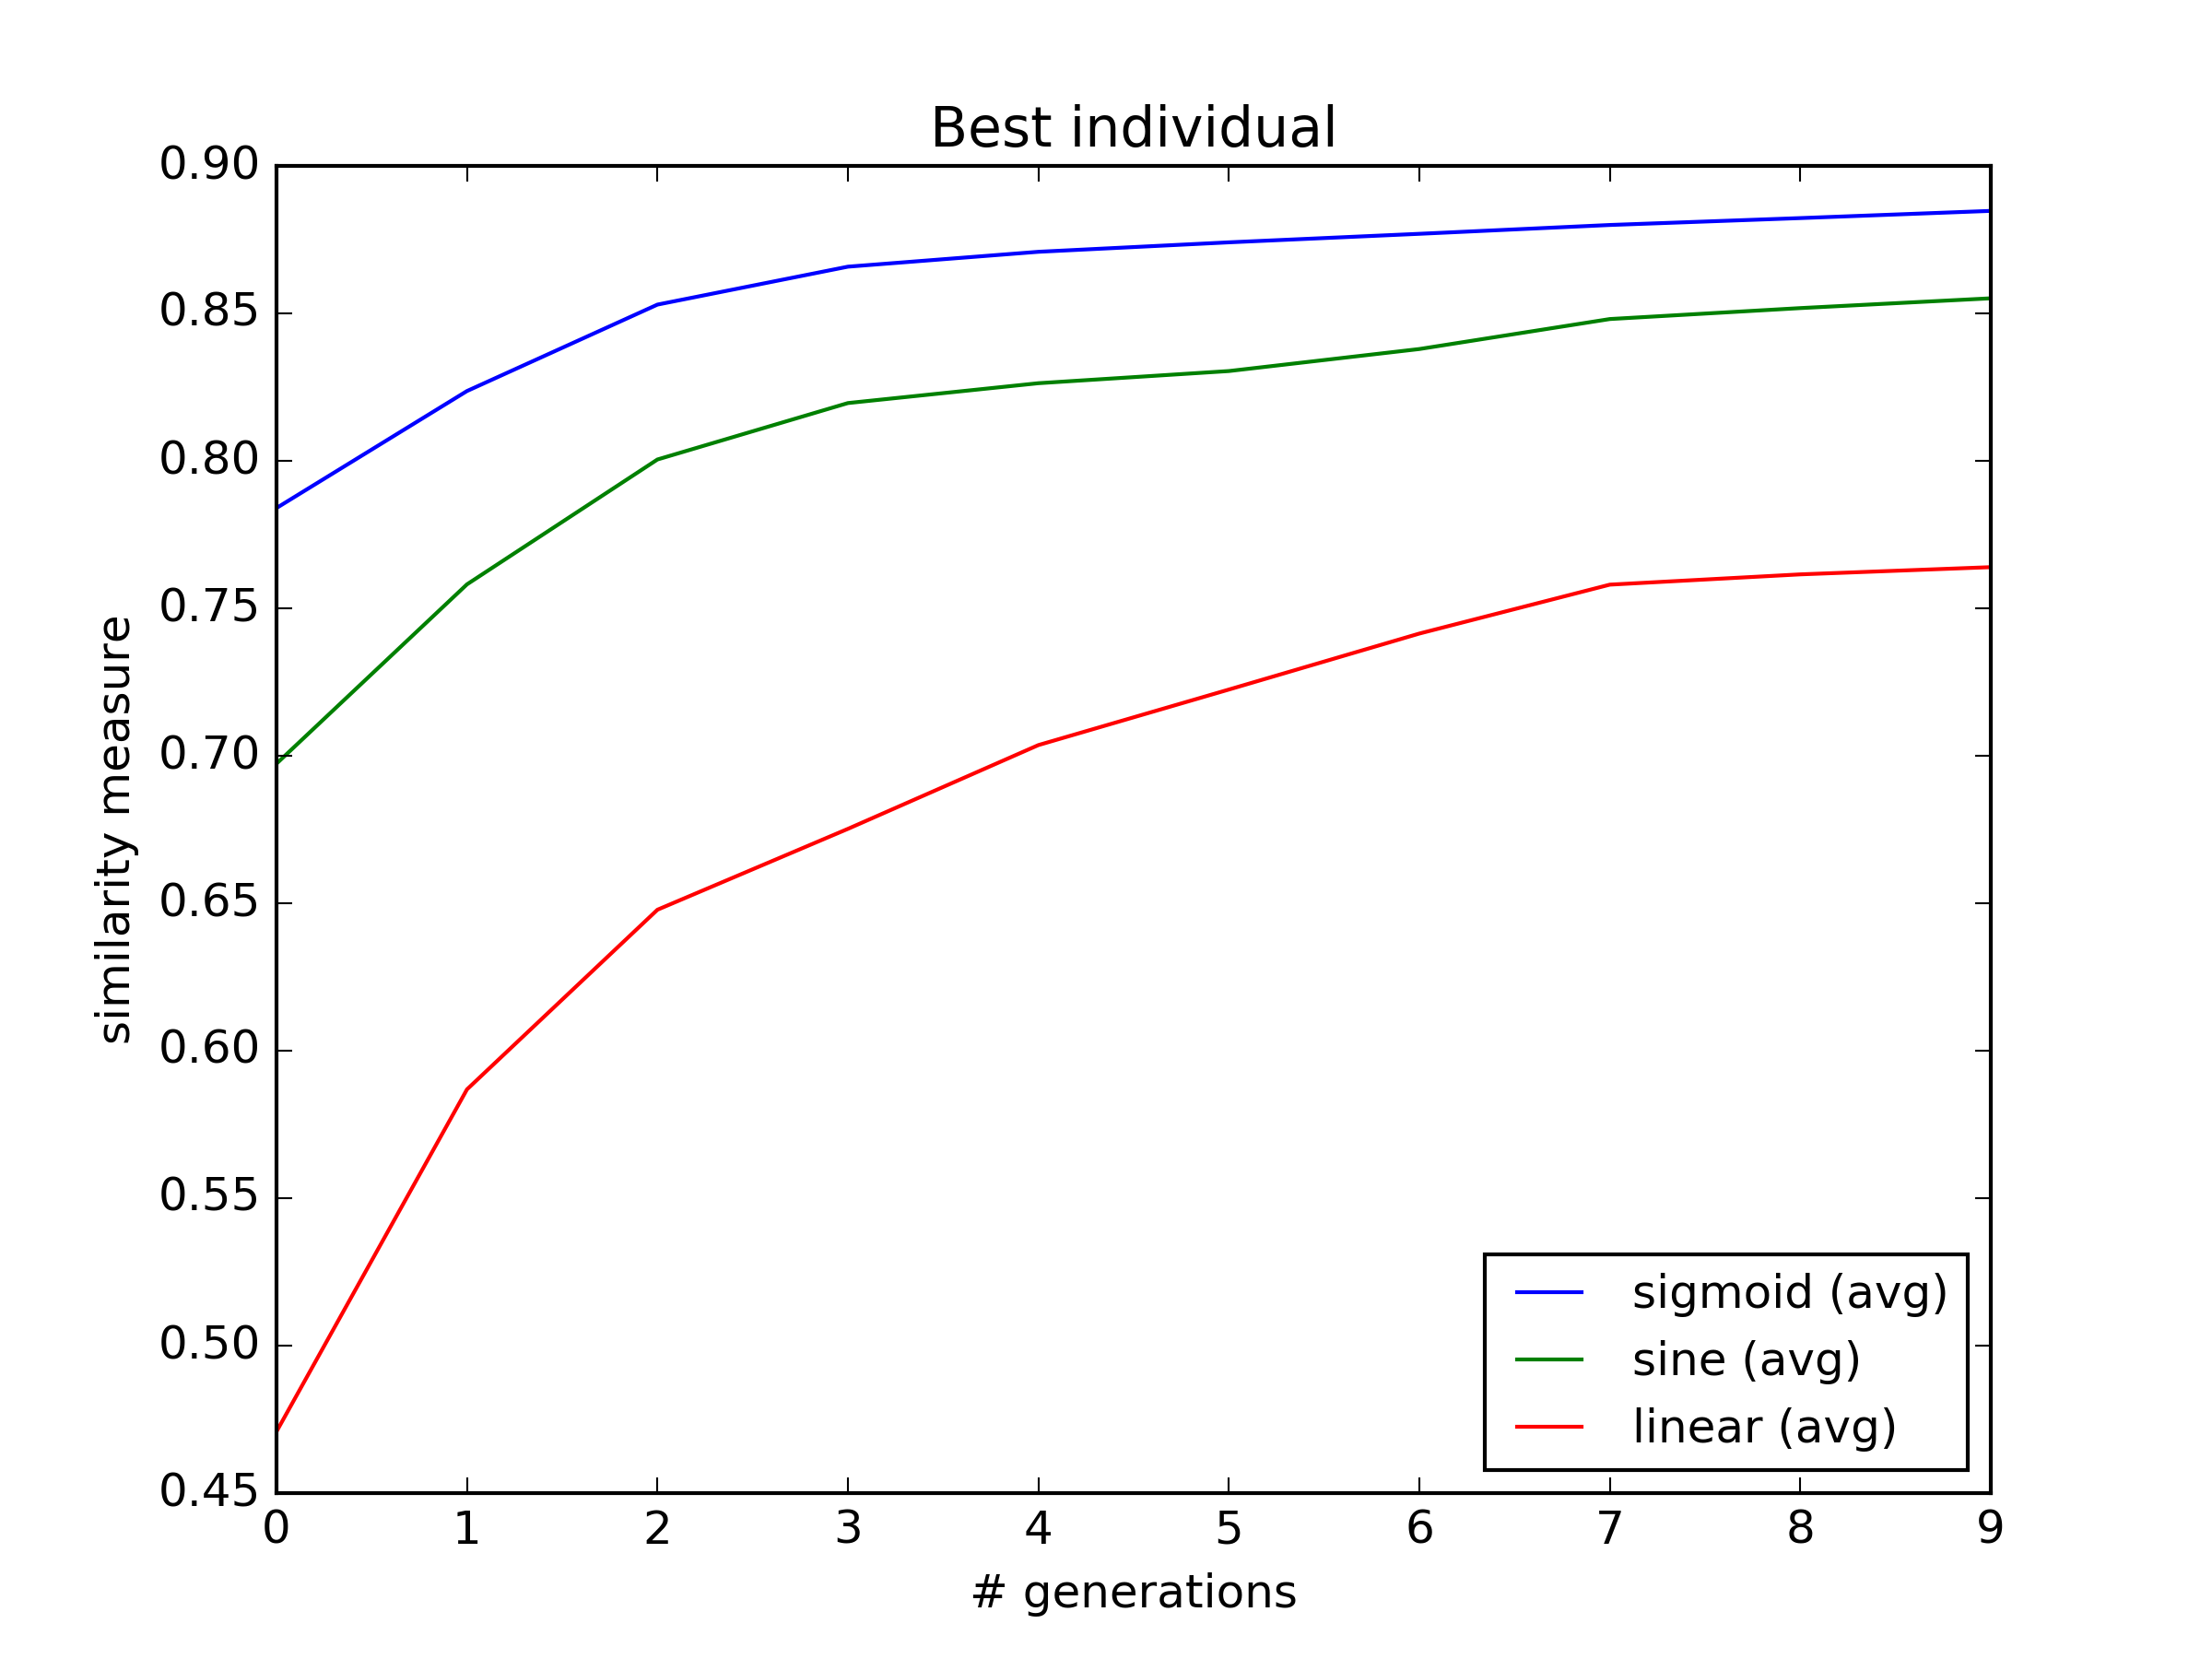
\includegraphics[width=0.99\textwidth]{08_plot_output_activation_functions_avg_experiment1}
    \caption{Average similarity over 20 runs. Three different output activation functions are compared}
    \label{fig:plot_output_activation_functions_avg_experiment1}
\end{figure}

\subsection{Evaluation of output sound}
The results are as expected: The amplitude of the best output sound is quite similar to the amplitude of the target sound. Figure 4.2 TODO shows this in that waveform C looks like waveform A. However, the bass drum hits in the output are not quite as strong as in the target sound. This is because the mfcc\_0 feature is not a pure amplitude measure and yields lower values for the bass drum hits than for the snare hits. Figure 4.3 shows this. Further, the distinction between bass drum and snare drum in the output sound is nonexistent. That will be dealt with in experiment 2, by adding more features for neural input and similarity measure.

\begin{figure}[h]
    \centering
    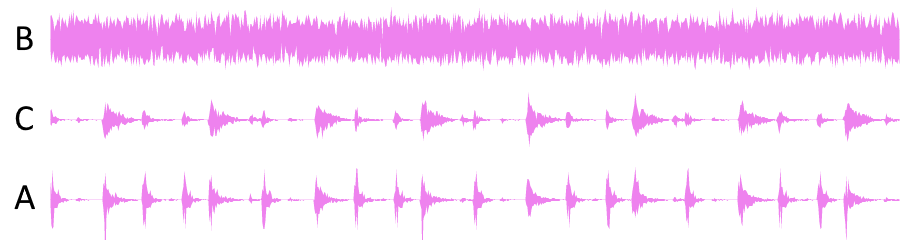
\includegraphics[width=0.99\textwidth]{09_experiment1_waveform_comparison}
    \caption{Waveform visualizations of input sound (B), output sound (C) and target sound (A).}
    \label{fig:experiment1_waveform_comparison}
\end{figure}

\begin{figure}[h]
    \centering
    
\includegraphics[width=0.99\textwidth]{10_drums_mfcc0_horizon_experiment1}
    \caption{The mfcc\_0 feature series of the drums sound visualized in a horizon graph}
    \label{fig:drums_mfcc0_horizon_experiment1}
\end{figure}